\documentclass{article}

% packages
\usepackage{amsmath, amsthm, thmtools, amsfonts, amssymb, luacode, catchfile, tikzducks, hyperref, ifthen}
\ifcsname c@kobocompile\endcsname
	\usepackage[a5paper, total={1072pt, 1448pt}, margin=10pt, includeheadfoot]{geometry} % set page margins
\else
	\usepackage[a4paper, margin=50pt, includeheadfoot]{geometry}
\fi
\usepackage[shortlabels]{enumitem}
\usepackage[skip=3pt, indent=0pt]{parskip}

% language
\usepackage[bidi=basic, layout=tabular, provide=*]{babel}
\ifcsname c@english\endcsname
	\babelprovide[main, import]{english}
\else
	\babelprovide[main, import]{hebrew}
	\babelprovide{rl}
\fi
%\babelfont{rm}{Libertinus Serif}
\babelfont{rm}[Renderer=Harfbuzz]{Libertinus Serif}
\babelfont{sf}{Libertinus Sans}
\babelfont{tt}{Libertinus Mono}

% style
\AddToHook{cmd/section/before}{\clearpage}	% Add line break before section
\linespread{1.3}
\setcounter{secnumdepth}{0}		% Remove default number tags from sections, this won't do well with theorems
\AtBeginDocument{\setlength{\belowdisplayskip}{3pt}}
\AtBeginDocument{\setlength{\abovedisplayskip}{3pt}}
\graphicspath{ {../images/} }

% operators
\DeclareMathOperator\cis{cis}
\DeclareMathOperator\Sp{Sp}
\DeclareMathOperator\tr{tr}
\DeclareMathOperator\im{Im}
\DeclareMathOperator\re{Re}
\DeclareMathOperator\diag{diag}
\DeclareMathOperator*\lowlim{\underline{lim}}
\DeclareMathOperator*\uplim{\overline{lim}}
\DeclareMathOperator\rng{rng}
\DeclareMathOperator\Sym{Sym}
\DeclareMathOperator\Arg{Arg}
\DeclareMathOperator\Log{Log}
\DeclareMathOperator\dom{dom}
\DeclareMathOperator\supp{Supp}
\DeclareMathOperator\var{Var}
\DeclareMathOperator\cov{Cov}

% commands
%\renewcommand\qedsymbol{\textbf{מש''ל}}
%\renewcommand\qedsymbol{\fbox{\emoji{lizard}}}
\newcommand{\Aa}[0]{\mathcal{A}}
\newcommand{\Bb}[0]{\mathcal{B}}
\newcommand{\CC}[0]{\mathbb{C}}
\newcommand{\Cc}[0]{\mathcal{C}}
\newcommand{\EE}[0]{\mathbb{E}}
\newcommand{\FF}[0]{\mathbb{F}}
\newcommand{\Ff}[0]{\mathcal{F}}
\newcommand{\Ii}[0]{\mathcal{I}}
\newcommand{\Gg}[0]{\mathcal{G}}
\newcommand{\Ll}[0]{\mathcal{L}}
\newcommand{\Mm}[0]{\mathcal{M}}
\newcommand{\NN}[0]{\mathbb{N}}
\newcommand{\Nn}[0]{\mathcal{N}}
\newcommand{\PP}[0]{\mathbb{P}}
\newcommand{\Pp}[0]{\mathcal{P}}
\newcommand{\QQ}[0]{\mathbb{Q}}
\newcommand{\RR}[0]{\mathbb{R}}
\newcommand{\Rr}[0]{\mathcal{R}}
\newcommand{\Ss}[0]{\mathcal{S}}
\newcommand{\TT}[0]{\mathbb{T}}
\newcommand{\Uu}[0]{\mathcal{U}}
\newcommand{\Vv}[0]{\mathcal{V}}
\newcommand{\Ww}[0]{\mathcal{W}}
\newcommand{\ZZ}[0]{\mathbb{Z}}
\newcommand{\acts}[0]{\circlearrowright}
\newcommand{\explain}[2] {
	\begin{flalign*}
		 && \text{#2} && \text{#1}
	\end{flalign*}
}
\newcommand{\maketitleprint}[0]{ \begin{center}
	%\begin{tikzpicture}[scale=3]
	%	\duck[graduate=gray!20!black, tassel=red!70!black]
	%\end{tikzpicture}	
	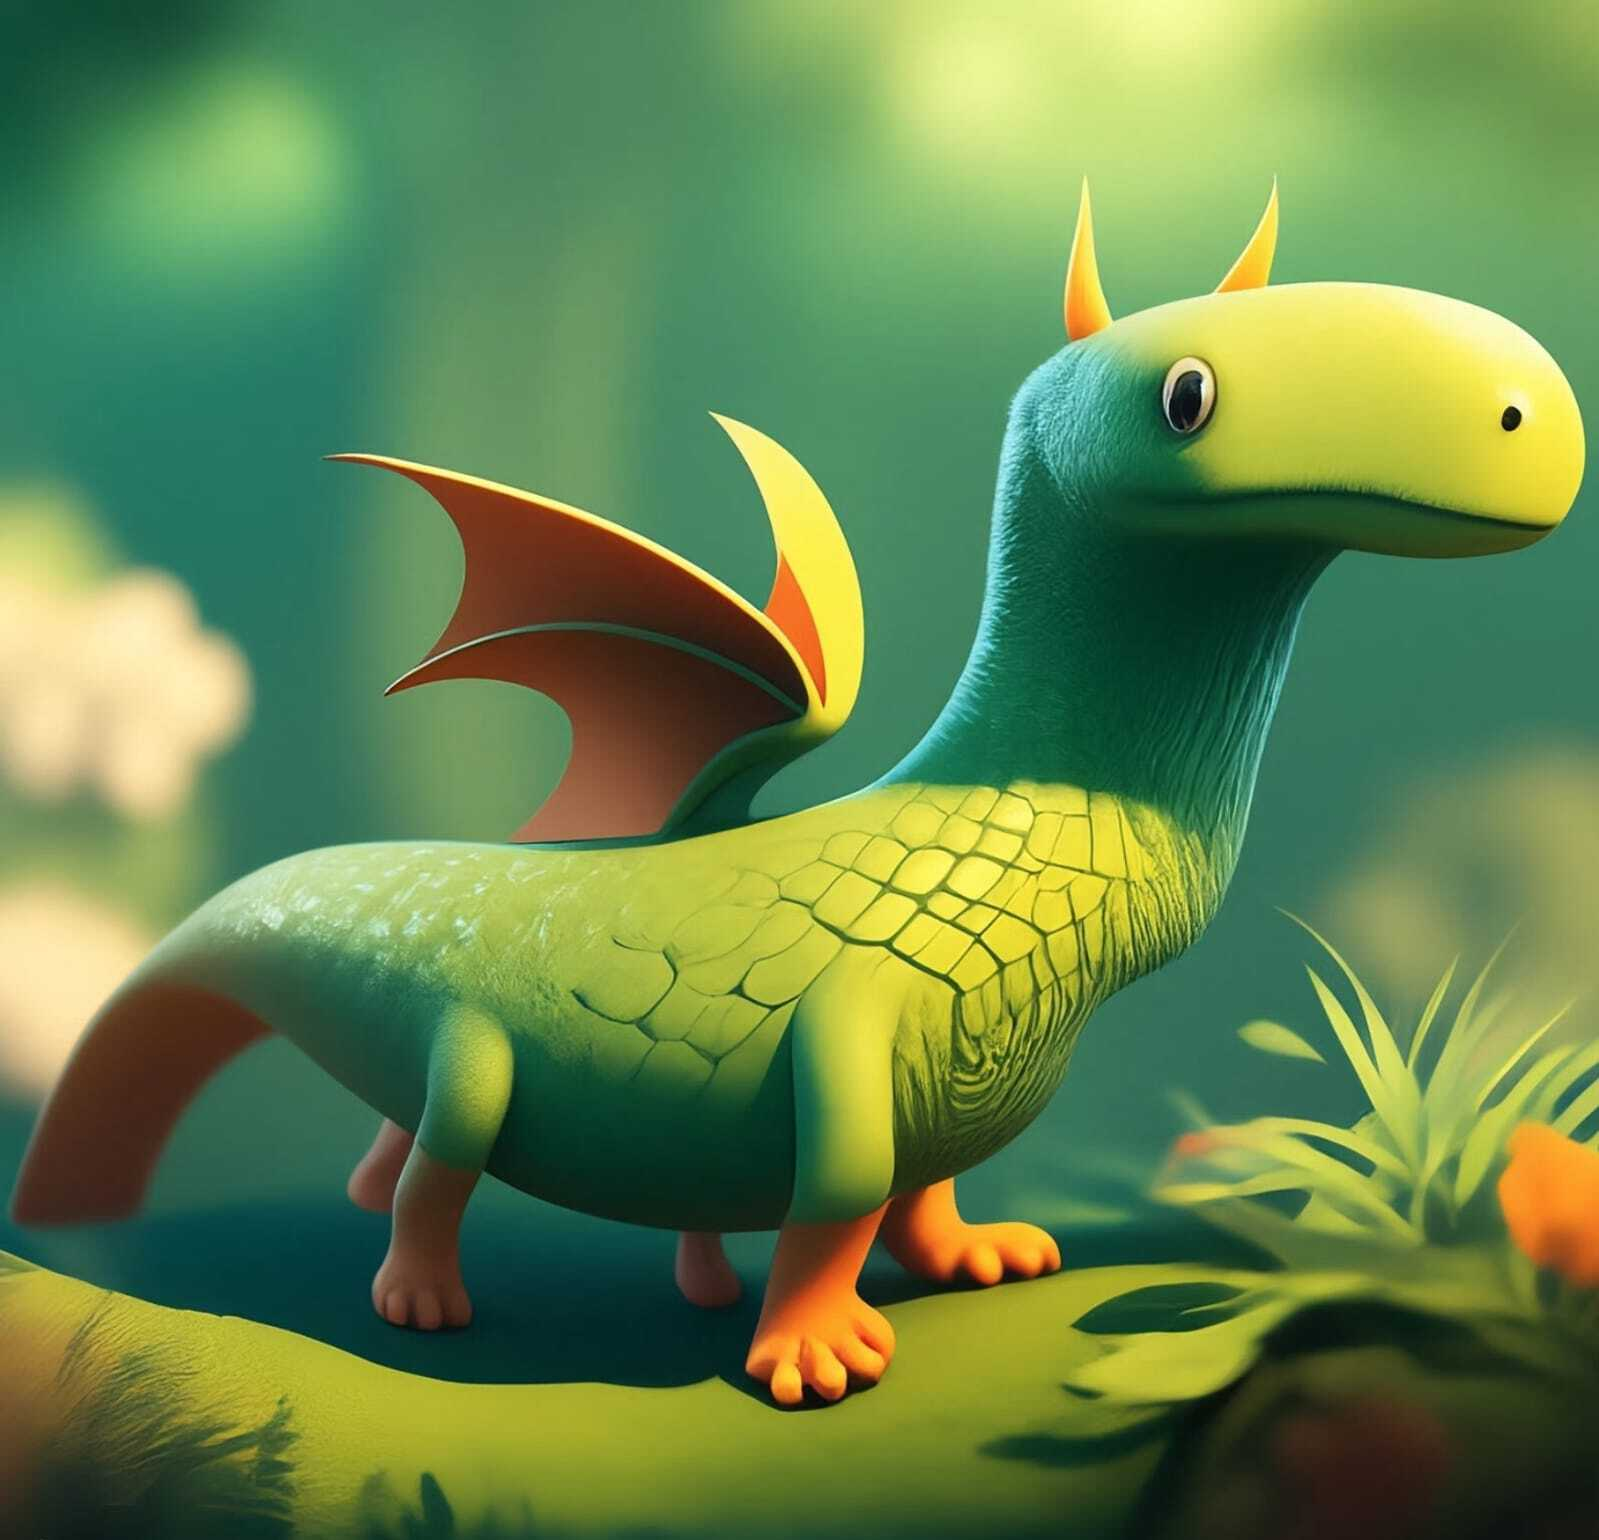
\includegraphics[width=6cm]{cover}
\end{center}
}

% theorem commands
\newtheoremstyle{c_remark}
	{}	% Space above
	{}	% Space below
	{}% Body font
	{}	% Indent amount
	{\bfseries}	% Theorem head font
	{}	% Punctuation after theorem head
	{.5em}	% Space after theorem head
	{\thmname{#1}\thmnumber{ #2}\thmnote{ \normalfont{\text{(#3)}}}}	% head content
\newtheoremstyle{c_definition}
	{3pt}	% Space above
	{3pt}	% Space below
	{}% Body font
	{}	% Indent amount
	{\bfseries}	% Theorem head font
	{}	% Punctuation after theorem head
	{.5em}	% Space after theorem head
	{\thmname{#1}\thmnumber{ #2}\thmnote{ \normalfont{\text{(#3)}}}}	% head content
\newtheoremstyle{c_plain}
	{3pt}	% Space above
	{3pt}	% Space below
	{\itshape}% Body font
	{}	% Indent amount
	{\bfseries}	% Theorem head font
	{}	% Punctuation after theorem head
	{.5em}	% Space after theorem head
	{\thmname{#1}\thmnumber{ #2}\thmnote{ \text{(#3)}}}	% head content

\ifcsname c@english\endcsname
	\theoremstyle{plain}
	\newtheorem{theorem}{Theorem}[section]
	\newtheorem{lemma}[theorem]{Lemma}
	\newtheorem{proposition}[theorem]{Proposition}
	\newtheorem*{proposition*}{Proposition}
	%\newtheorem{corollary}[theorem]{אין חלופה עברית}

	\theoremstyle{definition}
	\newtheorem{definition}[theorem]{Definition}
	\newtheorem*{definition*}{Definition}
	\newtheorem{example}{Example}[section]
	\newtheorem{exercise}{Exercise}[section]

	\theoremstyle{remark}
	\newtheorem*{remark}{Remark}
	\newtheorem*{solution}{Solution}
	\newtheorem{conclusion}[theorem]{Conclusion}
	\newtheorem{notation}[theorem]{Notation}
\else
	\theoremstyle{c_plain}
	\newtheorem{theorem}{משפט}[section]
	\newtheorem{lemma}[theorem]{למה}
	\newtheorem{proposition}[theorem]{טענה}
	\newtheorem*{proposition*}{טענה}
	%\newtheorem{corollary}[theorem]{אין חלופה עברית}

	\theoremstyle{c_definition}
	\newtheorem{definition}[theorem]{הגדרה}
	\newtheorem*{definition*}{הגדרה}
	\newtheorem{example}{דוגמה}[section]
	\newtheorem{exercise}{תרגיל}[section]

	\theoremstyle{c_remark}
	\newtheorem*{remark}{הערה}
	\newtheorem*{solution}{פתרון}
	\newtheorem{conclusion}[theorem]{מסקנה}
	\newtheorem{notation}[theorem]{סימון}
\fi

% Questions related commands
\newcounter{question}
\setcounter{question}{1}
\newcounter{sub_question}
\setcounter{sub_question}{1}

\ifcsname c@english\endcsname
	\newcommand{\question}[1][0]{
		\ifthenelse{#1 = 0}{}{\setcounter{question}{#1}}
		\section{Question \arabic{question}}
		\addtocounter{question}{1}
		\setcounter{sub_question}{1}
	}

	\newcommand{\subquestion}[1][0]{
		\ifthenelse{#1 = 0}{}{\setcounter{sub_question}{#1}}
		\subsection{Part \alph{sub_question}}
		\addtocounter{sub_question}{1}
	}
\else
	\newcommand{\question}[1][0]{
		\ifthenelse{#1 = 0}{}{\setcounter{question}{#1}}
		\section{שאלה \arabic{question}}
		\addtocounter{question}{1}
		\setcounter{sub_question}{1}
	}

	\newcommand{\subquestion}[1][0]{
		\ifthenelse{#1 = 0}{}{\setcounter{sub_question}{#1}}
		\subsection{סעיף \localecounter{letters.gershayim}{sub_question}}
		\addtocounter{sub_question}{1}
	}
\fi

% import lua and start of document
\directlua{common = require ('../common')}

\GetEnv{AUTHOR}

% headers
\author{\AUTHOR}
\date\today

\title{פתרון מטלה 07 --- מבוא לטופולוגיה, 80516}
% chktex-file 9
% chktex-file 17

\begin{document}
\maketitle
\maketitleprint[purple]

\question{}
תהי $f : X = [0, 1] \to {[0, 1]}^2 = Y$ רציפה ועל.
נראה ש־$f$ אינה חד־חד ערכית.
\begin{proof}
	נניח בשלילה ש־$f$ גם חד־חד ערכית.
	נבחין כי שני המרחבים הם מרחבי בייר ממשפט הקטגוריה של בייר, כלומר אין לקבוצות מקטגוריה שנייה פנים.
	בנוסף אנו יודעים כי שני המרחבים הם האוסדורף וקומפקטיים ולכן $f$ סגורה ונובע שהיא הומיאומורפיזם.

	נגדיר $Z = \{ \frac{1}{2} \} \times [0, 1] \subseteq Y$, זוהי קבוצה דלילה, זאת שכן $\overline{Z} = Z$ אבל אין בה אף כדור פתוח.
	לכן גם $f^{-1}(Z) \subseteq X$ היא קבוצה דלילה.
	בפרט היא מקטגוריה ראשונה ולכן $X_0 = X \setminus f^{-1}(Z)$ היא מקטגוריה שנייה ובעלת פנים ריק.
	אבל $Y \setminus Z$ מורכבת משני רכיבי קשירות מסילתית ולכן גם $X_0$ מורכבת משני רכיבי קשירות מסילתית ובפרט מורכבת משני קטעים פתוחים ב־$[0, 1]$.
	בפרט הפנים של קטעים אלה לא ריק, וקיבלנו סתירה.
\end{proof}

\question[3]
יהי $X$ מרחב טופולוגי,
$A \subseteq X$ תיקרא $G_{\delta}$ ב־$X$ אם היא חיתוך בן־מניה של פתוחות מ־$X$.

\subquestion{}
יהי $X$ מרחב בייר ותהי $A \subseteq X$ קבוצה $G_{\delta}$ צפופה ב־$X$.
נראה ש־$A$ מרחב בייר.
\begin{proof}
	נניח ש־$B \subseteq A$ פתוחה, אז $B' \subseteq X$ פתוחה כך ש־$B' \cap A = B$.
	אבל בהתאם $B'$ היא קבוצה $G_{\delta}$ ב־$X$.
	עתה נניח ש־$B_{\alpha}$ קבוצות פתוחות וצפופות ב־$A$, אז $B_{\alpha}' \subseteq X$ פתוחות וצפופות ב־$X$ כך ש־$B_{\alpha} = A \cap B_{\alpha}'$, לכל $\alpha \in \NN$.
	$X$ הוא מרחב בייר ולכן $\bigcap_{\alpha \in \NN} B_{\alpha}'$ צפופה ב־$X$ ובפרט $A \cap \bigcap_{\alpha \in \NN} B_{\alpha}' = \bigcap_{\alpha \in \NN} B_{\alpha}$ צפופה ב־$A$, ולכן $A$ מרחב בייר.
\end{proof}

\subquestion{}
נמצא דוגמה למרחב בייר $X$ ו־$A \subseteq X$ קבוצת $G_{\delta}$ שאינה מרחב בייר.
\begin{solution}
	נגדיר $X = (\RR \times (0, \infty)) \cup (\QQ \times \{0\})$.
	המרחב $\HH = \{ (x, y) \in \RR^2 \mid y \ge 0 \}$ הוא מרחב מטרי שלם ולכן בייר.
	הקבוצה $\HH$ כמובן פתוחה וכן לכל רציונלי גם $(q, 0) \in B((q, 1), 1)$ ולכן נוכל להסיק ש־$X$ היא $G_{\delta}$ ב־$\HH$ וצפופה ולכן מרחב בייר.

	נגדיר עתה $A = \QQ \times \{ 0 \}$.
	זוהי קבוצה סגורה ב־$X$ כ־$\partial \HH$, ומאפיון קבוצות סגורות במרחבים מטריים נובע שגם $G_{\delta}$.
	לעומת זאת $A$ היא לא קבוצת בייר כטענה מהתרגול, ולכן מהווה דוגמה כפי שרצינו.
\end{solution}

\question{}
\subquestion{}
יהי $X$ מרחב בייר $T_1$ עם כמות בת־מניה של נקודות.
נראה שקיימת ב־$X$ נקודה מבודדת.
\begin{proof}
	אם קיים יחידון פתוח ב־$X$ אז סיימנו, לכן נניח שאין כאלה.
	יהי $x_0 \in X$, אז לכל $y \ne x_0$ קיימת סביבה פתוחה $y \in U_y \subseteq X$ כך ש־$x \notin U_y$, זאת כנביעה מ־$T_1$.
	מסגירות לאיחודים נסיק ש־$\bigcup_{y \ne x_0} U_y$ קבוצה פתוחה, ולכן $\{ x_0 \}$ קבוצה סגורה.
	אז נובע ש־$\{ x_0 \}$ היא קבוצה דלילה לכל $x_0 \in X$.
	נסיק ש־$X = \bigcup_{x \in X} \{ x \}$ והעובדה ש־$X$ בת־מניה כי היא קבוצה מקטגוריה ראשונה.
	אבל $X$ מרחב בייר ולקבוצות מקטגוריה ראשונה אין פנים, כלומר $X^\circ = X = \emptyset$ בלבד.
	אבל $|X| = \aleph_0$ בסתירה ל־$X = \emptyset$, ולכן נסיק שקיים יחידון פתוח.
\end{proof}

\subquestion{}
נראה ש־$\RR$ אינו איחוד בן־מניה זר של קטעים סגורים וחסומים. \\
כלומר עבור קטעים זרים וחסומים $[a_n, b_n]$ ל־$n \in \NN$ מתקיים $\RR \setminus \bigcup_{n \in \NN} [a_n, b_n] \ne \emptyset$.
\begin{proof}
	נניח בשלילה שקיימים קטעים כאלה, ונגדיר $X = \bigcup_{n \in \NN} \{ a_n, b_n \}$.
	הקבוצה $X$ היא קבוצה בת־מניה ו־$T_1$ מזרות הקטעים.
	זהו גם מרחב מטרי כמרחב המושרה מ־$\RR$, ומדיסקרטיות הוא אף שלם, ולכן ממשפט הקטגוריה של בייר נסיק שהוא מרחב בייר.
	נובע אם כך מסעיף א' שקיימת ב־$X$ נקודה מבודדת.
	נניח בלי הגבלת הכלליות ש־$a_l$ היא הנקודה הזו, לכן נובע שיש סביבה פתוחה של $a_l$ בה אין נקודות $b_n$ לאף $n$, כלומר $(a_l - \epsilon, a_l) \cap [a_l, b_l]$ קבוצה ריקה, ובפרט $a_l - \epsilon$ לא נמצאת באף קטע.
\end{proof}

\end{document}
